% Bhaskar
% biological-perspectives-evolvability.tex
%%%%%%%%%%%%%%%%%%%%%%%%%%%%%%%%%%%%%%%%%%%%%%%%%%%%%%%%%%%%%%%%%%%%%%%%%%%%%%%%%%
% revision status as of 2026_03_03 (Planning to get to incorporating remaining comments/suggestions and references today but might not be done before 1300hr sorry!)
% - [x] accept or reject all track changes
% - [-] incorporate review comments
%    - don't worry about clearing all comments
% - [x] incorporate reference suggestions
% - [ ] cross-cutting revision objectives (see email)
% - [ ] other planned changes or refinements (if any)
% for revision status, mark - for partial or x for complete
% any free-form comments on planned/completed revisions are helpful too!
% --------------------------------------------------------------------------------
% draft status: Complete draft as of 2025_12_1   <---------- fill me in!
% Aiming to get to complete draft by 2025/11/28
% pick one of: outline, partial draft, rough draft, complete draft
% where rough draft indicates that major points are hit,
% but still working on changes or improvements in refining the text
%%%%%%%%%%%%%%%%%%%%%%%%%%%%%%%%%%%%%%%%%%%%%%%%%%%%%%%%%%%%%%%%%%%%%%%%%%%%%%%%%%

\section{Adaptive Landscapes}
\label{sec:evolvability}

\begin{figure}
    \centering
    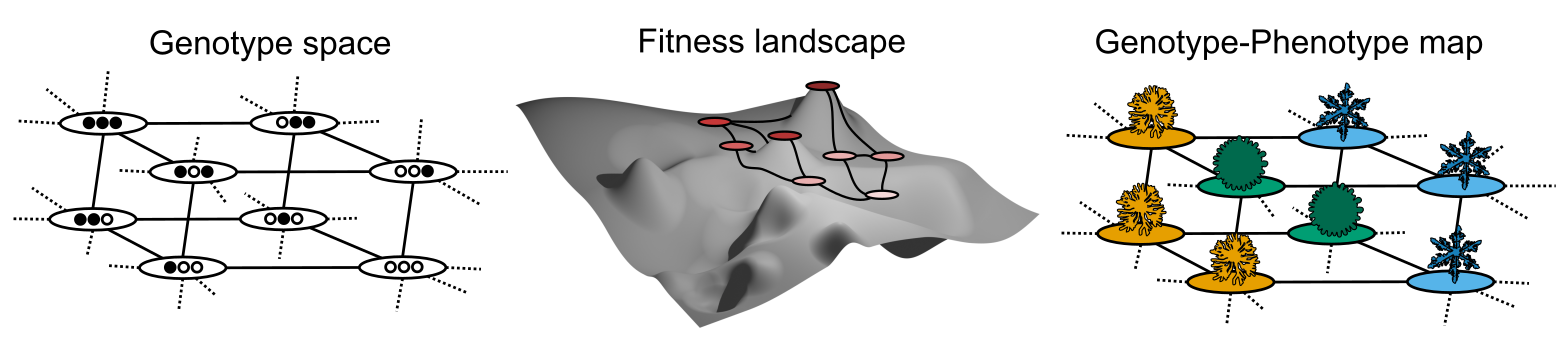
\includegraphics[width=1.0\linewidth]{img/fitness_landscapes.png}
    \caption{%
\textbf{Adaptive Landscapes}.
The \textit{genotype space} (left) is a network of genotypes, with edges connecting genotypes that differ by a single mutation.
A \textit{fitness landscape} (middle) is induced on this space when each genotype is assigned a value denoting its reproductive success in an environment.
Alternatively, the genotypes may be assigned ``phenotypes'' that denote expressed traits, producing a \textit{genotype-phenotype map} (right)
}
\label{fig:fitness_landscapes}
\end{figure}


% \begin{itemize}
% \item \citet{eppstein2016quantifying} use an empirical fitness landscape for $\beta$-lactam antibiotic resistance to quantify deception in evolutionary search, applying evolutionary-computation diagnostics to a biologically grounded mutational graph.
% Their case study shows that real drug-resistance landscapes can exhibit substantial deception, and they introduce a framework for characterizing how landscape topography misleads adaptive walks toward suboptimal peaks.
% \item \citet{schaper2014arrival} argue that strong bias in genotype-phenotype maps --- where some phenotypes are encoded by exponentially more genotypes than others --- systematically channels populations toward ``frequent'' phenotypes regardless of their fitness.
% They show via theory and simulation that this ``arrival of the frequent'' can trap populations on locally suboptimal phenotypes long before selection can act, complicating the standard ``survival of the fittest'' picture of adaptation.
% \item \citet{fragata2019evolution} review recent theoretical and empirical progress in fitness landscape theory, surveying how high-throughput measurements of landscape topography are reshaping understanding of epistasis, ruggedness, and accessibility of adaptive paths.
% The review argues that landscape thinking remains a powerful organizing framework for evolutionary biology, but emphasizes that effective use requires integrating empirical landscape data with population-genetic models of mutation, drift, and selection.
% \item \citet{altenberg1995genome} evelops a theoretical framework in which genome growth via gene duplication interacts with the structure of the genotype-phenotype map to drive the evolution of evolvability.
% He introduces ``constructional selection,'' a second-order process in which newly added genes are retained when their pleiotropic effects tend to produce fitness improvements, thereby biasing genome architecture over time toward representations more conducive to adaptive evolution.
% \item mystery citations \citep{schmitt2003theory,andre2001improvement,bongard2010guarding,pandey2014comparative,crepinsek2013exploration,iwasa2004stochastic,peniston2020environmental,steinberg2016environmental,devos2015breaking}.
% \end{itemize}

The fundamental property differentiating evolution from random search is mutational locality --- the tendency for mutation to preserve some aspects of phenotypes \citep{maynardsmith1970natural,galvanlopez2011defining,ashlock2012representation,back1996evolutionary,foster2001evolutionary,richter2014fitness}.

The property stems from the geometry from genotype space, which arranges all possible genetic sequences into sets of mutational neighbors  \citep{fragata2019evolution,castle2021towards}.
While classic visualizations often cast it in one or two dimensions \citep{mcleish2015there,greenbury2022structure,gordon1994evolution,gavrilets1997evolution}, genotype space is more accurately conceptualized as a dense network where each genotype is surrounded by numerous single-mutant neighbors (Figure \ref{fig:fitness_landscapes}, left).
The extreme size and high dimensionality and reason about and even visualize \citep{dolsonTODO}, with matters is further complicated by recombination processes that can allow far-reaching jumps \citep{li2024rapid,doerr2008crossover,fogel1994effectiveness}.

The second major factor distinguishing evolution from random search is variation in fitness across genotype space, which strongly biases population trajectories.
Thus, genotype space is often viewed through the lens of a fitness landscape, where assigns each genotype a corresponding fitness value (Figure \ref{fig:fitness_landscapes}, middle).
In scenarios where fitness values may change over time depending on ecological or environmental factors \citep{olson2014dynamic,kaplan2008end,dolson2021digital}, a fitness landscape may instead be termed a ``fitness seascape'' \citep{cairns2022strong,mustonen2009fitness}.

A useful decomposition of adaptive landscapes, arising in both evolutionary computation and evolutionary biology, is the genotype-phenotype map \citep{ahnert2017structural,aguilar2018architecture,stadler2003landscapes}.
In biology, phenotype (the observable traits of an organism) can often be more readily and consistently observed than fitness, making it a more tractable target of study \citep{chen2022environmental,ahnert2017structural,wagner2011pleiotropic,aguilar2018architecture}.
In evolutionary computation, discussion of the genotype-phenotype map typically revolves around the theme of indirect encoding, where a genotype space with desirable properties is constructed by defining a mapping function into phenotype (i.e., solution) space \citep{stanley2007compositional,stanley2003taxonomy,stanley2009hypercubebased,clune2011performance,kitano1990designing,hornby2002creating}.k

\subsection{Ruggedness}

A key property of such a landscape is its ``rugedness'' \citep{papkou2023rugged,reidys2001neutrality} --- the extent to which ``peaks'' and ``valleys'' arise that constrain evolutionary exploration \citep{martin2013multiple,steinberg2016environmental}.
This ruggedness makes it difficult for adaptive evolution to explore the genotype space exhaustively, as populations may get stuck on locally optimal peaks \citep{li2025probability,bank2022epistasis,neidhart2014adaptation}.
If most adjacent mutations are deleterious, it severely limits the ability of the population to explore the genotype space \citep{orr2005genetic,bershtein2008advances}.
In evolutionary computation, this can contribute to the challenge of \textit{premature convergence}, where a population reaches a local optimum but not a global optimum.

\subsection{Neutrality}

Another geometric property of interest in mutational landscapes is neutral networks, which can connect ``neutrally'', without any effect on phenotypes or fitness and promote exploration and long-term innocations \citep{reidys2001neutrality,ahnert2017structural,croitoru2022punctuated,galvanlopez2011neutrality,jorg2008neutral,huynen1996smoothness,shackleton2000investigation,huynen1996exploring,amitai2007latent,banzhaf2006evolution,hu2025neutrality}.
Neutral networks have also been connected to \textit{mutational robustness} as a genotype within a neutral network can acquire many successive mutations without any apparent effect on fitness \citep{van1999neutral}.
This process has been used to resolve a long debate on tradeoffs between robustness and evolvability in such genotype spaces --- mutational robustness may inhibit evolutionary innovation on short time scales but can promote it over the long term \citep{wagner2008robustness,wagner2013robustness,masel2010robustness,hu2018neutrality}.
The degree to which a genotype-phenotype map allows for neutral \citep{kimura1983neutral,kimura1991neutral} (or nearly neutral \citep{ohta1992nearly,ohta2002near}) mutations greatly assists a population in escaping local optima, since selection is less able to prevent exploration \citep{oliveto2017how}.
Neutral networks complement the dimensional property of genotype space,
Thus, while genotype space is combinatorially vast, it  through only a few mutational steps, especially in spaces with a high dimensionality \citep{franke2011evolutionary} which can make it is possible to more easily reach global optima.

\subsection{Evolvability}

In evolutionary computation, the genotype-phenotype map is widely discussed in the context of the problem of evolvability.

Evolvability refers to
In a biological context, evolvability is defined as the capacity of a population to generate heritable phenotypic variation that facilitates adaptive evolution \citep{payne2018causes,kirschner1998evolvability}.
While a variety of mechanisms or facets have been brought to evolvability \citep{clune2008natural,hu2010evolvability,altenberg1994evolution,mengistu2016evolvability,riederer2022capturing}, it is typically thought of as related to the local structure of the fitness landscape defined with respect to available mutations \citep{wagner2017information,wagner2023evolvability}.

A key distinction in the approach arises because of the artificial nature of EC systems.
Because EC systems represent a of independent originations under bespoke rules,
Owing to the capability to before , evolutionary computation genotype-phenotype maps --- much less, maps with strong evolvability --- do not come baked into evolutionary computation \textit{a priori} \citep{kirschner1998evolvability}.
A typical EC framing defines evolvability as the genotype space as containing viable and novel solutions \citep{tarapore2015evolvability}.

As such, EC research has invested significant effort in teasing apart how the properties of a genotype-phenotype map influence outcomes from adaptive evolution \citep{banzhaf1994genotypephenotypemapping,hu2010evolvability,whigham2017mapping}.
On-line optimization of parameters during evolutionary searches is also a promising area of study when trying to overcome the limits of a given representation \citep{dang2016selfadaptation}.
Alternately, restarts or stochastic algorithms that can move vast distances in the genotype space in a few steps are sometimes necessary to sample the solution space somewhat exhaustively \citep{fogel1994introduction,fouskakis2002stochastic,kirkpatrick1983optimization,de2015money,doerr2014impact}.
New algorithms may be selected for a given problem based on metaheuristic analyses that try to take these representations into account \citep{wang2018population}.

However, most effort goes into \textit{designing} evolvable adaptive landscapes.
The structure of the space is strongly tied to the data structure used to encode the solutions and is generally referred to as a \textit{representation} \citep{ashlock2012representation,rothlauf2003redundant, rothlauf2009representations,mitavskiy2003comparing}, which together with the mutation operator controls how EC explores new solutions \citep{stark2004rate}.

A particularly promising line of EC work has sprung up in investigating how to harness unsupervised learning (e.g., autoencoders, LLMs) to generate evolvable genotype-phenotype maps \citep{lehman2023evolution,moreno2018learning,bentley2022evolving,gaier2020discovering,wittenberg2023denoising}.
Under this framing, TODO

\subsection{Landscape Locality}

Unlike EC where the user can design a suitable representation and mutation operator, in nature the ``representation'' for an evolving population is fixed to DNA/RNA sequence space composed of the four nucleotide bases \citep{aguirre2018networked} (there is some potential to engineer it though, see \citet{zhang2015evolution}).
Because natural selection only operates on the current environment \citep{watson2016how}, whether it can allow optimization for long-term outcomes is heavily debated \citep{wagner2021adaptive,akay2016there,keller1999levels,altenberg1995genome}.
However, within the exponentially vast space of genotypes \citep{stadler2007fitness,de2014empirical}, evolution can exploit local structural features of the landscape in interesting ways \citep{kumawat2024evolution,barnett2025experimental,steinberg2016environmental,gupta2022hostparasite,ferrare2024evolution,pyo20Mutations can be considered ``evolvability enhancing'' if they provide access to later high fitness mutations, which are surprisingly abundant in biological fitness landscapes \citep{wagner2023evolvability} --- although the generality of this abundance remains to be explored \citep{ogbunugafor2023mutations}.

In a changing environment with varying requirement for survival \citep{bell2017evolutionary,bell2010fluctuating}, mutations may benefit a lineage directly, or with respect to an environment that is likely to appear in the future \citep{parter2008facilitated}.
These second-order effects, which run counter to the common adage of ``survival of the fittest,'' have received significant attention \citep{akay2016there} --- with an emerging view that, under certain conditions, evolution can act not just to optimize instantaneous fitness, but rather the long-term growth rate among competing lineages \citep{akay2016there,yoshimura1996evolution,yoshimura1991individual}.
For instance, in a changing environment, a high-fitness genotype may be out-competed by genotypes that are lower in fitness, but belong to a lineage that switches quickly between phenotypes adapted to alternate environments \citep{woods2011secondorder}.
The idea that mutation and selection can select for better long-term outcomes has been conclusively shown in both biological and computational evolving systems \citep{sung2012driftbarrier, wilke2001evolution, pyo2025evolutionary, wagner2021adaptive, akay2016there, keller1999levels, wagner2017information, kumawat2024evolution, barnett2025experimental, steinberg2016environmental, hayden2011cryptic, gupta2022hostparasite, zaman2014coevolution}.
It is plausible that certain selection schemes used regularly in EC are already good at optimizing lineage-level aggregate fitness, and at converging to high-fitness solutions \citep{hu2010evolvability,doncieux2020novelty,lehman2015enhancing}.
Systematic effort towards a taxonomy of second-order optimization protocols needs to be undertaken in future work \citep{gajewski2019evolvability,mengistu2016evolvability,hu2010evolvability}.
The above discussion on biological outcomes provides some hints to guide their design.

Regardless, some areas of genome space are likely to have different phenotypes available locally \citep{wagner2017information},
and recent work has shown that environmental change pushes populations to these boundaries where they can more freely mutate between alternate phenotypes \citep{kumawat2024evolution,barnett2025experimental,kussell2006polymerpopulation,ancel2005evolution}.
Further, the structure of the fitness landscape may limit the effectiveness of evolutionary control methods used to suppress the growth of harmful microbial populations or for directed evolution.
Environmental change induced deformations in the fitness landscape can push the population away from genotypes that are locally fit in a specific environment, which in turn allows the population to sample new genotypes in the landscape \citep{steinberg2016environmental}.
The role of such changing fitness landscapes, or seascapes, in EC optimization problems remains insufficiently explored \citep{grefenstette1999evolvability,richter2009detecting}.

Biologists have developed several useful measures to quantify the ease with which evolution can respond to changing environment selection.
For example, researchers have shown that abundant edge-flips in a fitness landscape --- i.e., single mutation edges that change the direction of adaptation between two mutants in two environments --- can allow us to predict the efficacy of intermittent antimicrobial therapy \citep{chen2024inverted}.
Similarly, a measure called the mutation effect reaction norm (Mu-RN) has been used to quantify the effect of mutations across environments \citep{ogbunugafor2022mutation}.
Work on drug resistant mutations has also formalized the idea of \textit{deception} on fitness landscapes, which is the presence of epistatic mutations that lead populations away from global optima \citep{eppstein2016quantifying,ogbunugafor2016competition}.
Biological literature thus provides an abundance of structural properties that can be directly translated into the EC domain to motivate the design of solution spaces and algorithms that leverage second-order outcomes of the evolutionary process.
Much unsolved work remains in predicting under what conditions a population will localize to different boundary genotypes, \citep{kussell2006polymerpopulation}, which may be an opportunity for EC to contribute.

A key challenge for these two fields is to unite their approach, to think about how learned encodings can translate into movement within a space rather than shaping a space.
However, we believe that application-oriented genetic programming and genetic algorithms have special value to offer in the realm of genotype-phenotype maps and evolvability.
On account of connections to machine learning concepts, the question of generalization and double-descent are unique ideas that have ben led into biology from EC.
Corresponding work in biology, however, is only fledgling.
Indeed, such work considering evolvability as an unsupervised learning process has notably already been driven forward through collaboration with evolutionary computation practitioners \citep{kouvaris2017evolution,szilagyi2020phenotypes}.
Some authors have suggested that the evolutionary process can in some ways ``learn'' from previous environments to prevent overfitting \citep{kouvaris2017evolution, watson2016how, watson2014evolution}.
This theory may help to explain, as well as to attain more evolvable mappings.
Boundary localization generalizes to representation-based framings of evolvability \citep{reisinger2006selecting} --- although this may unfold on a slower (e.g., macro) evolutionary timescale \citep{reznick2009darwin}.
Thus, using large search spaces with a \textit{representation optimizing} algorithm can give better overall results than directly trying to find a good representation \citep{hewlett2008optimization,gajewski2019evolvability,mengistu2016evolvability}.
